\documentclass{beamer}
\usepackage{fontspec}
\usepackage{subfig}
\usepackage{unicode-math}
\usepackage{tabularray}
\usepackage{ragged2e}
\usepackage{array}
\usepackage{setspace}
\usepackage{adjustbox}

\usetheme{metropolis}
\setbeamertemplate{footline}{}
\usefonttheme{professionalfonts}
\usefonttheme{serif}
\setmainfont{DejaVu Sans}
\setmathfont{XITS Math}


\title{Անտենաների թերությունների և ճառագայթվող էլեկտրամագնիսական դաշտի հետազոտումը ջերմաառաձգական օպտիկական ինդիկատորով մանրադիտակի օգնությամբ}
\author{Ուսանող՝ Սիմոնյանց Դավիթ}
\date{}

\newcommand{\sectslides}{0}
\newcounter{currslide}
\newcommand{\resetCountingSlides}[1]{
    \renewcommand{\sectslides}{#1}
    \setcounter{currslide}{1}
}
\newcommand{\countSlide}{\addtocounter{currslide}{1}}
\newcommand{\showSlide}{\thecurrslide/\sectslides}
\newcommand{\showCountSlide}{\showSlide \countSlide}
\newcommand{\frametitlecounted}[1]{\frametitle{#1 \hfill \fontsize{10}{10} \selectfont \showCountSlide}}


\begin{document}
\hyphenpenalty=10000
\exhyphenpenalty=10000

\begin{frame}
\vspace{4mm}
\begingroup
    \fontsize{9}{9} \selectfont ԵՐԵՎԱՆԻ ՊԵՏԱԿԱՆ ՀԱՄԱԼՍԱՐԱՆ \\ ՖԻԶԻԿԱՅԻ ԻՆՍՏԻՏՈՒՏ
\endgroup
\titlepage
\vspace{1cm}
\end{frame}

\resetCountingSlides{3}

\begin{frame}
\frametitlecounted{Ներածություն}

Անտենաները կարևոր դեր են խաղում հեռահաղորդակցության ոլորտում, հնարավորություն տալով հաղորդել և ընդունել էլեկտրամագնիսական ալիքներ։

\begin{figure}[ht]
  \centering
  \begin{adjustbox}{raise=20pt}
  \begin{minipage}[b]{0.45\linewidth}
    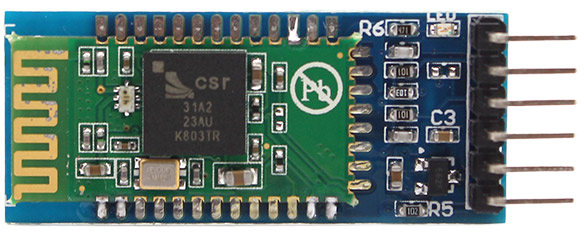
\includegraphics[width=\linewidth]{data/presentation/antenna-1.png}
  \end{minipage}
  \end{adjustbox}
  \hfill
  \begin{minipage}[b]{0.45\linewidth}
    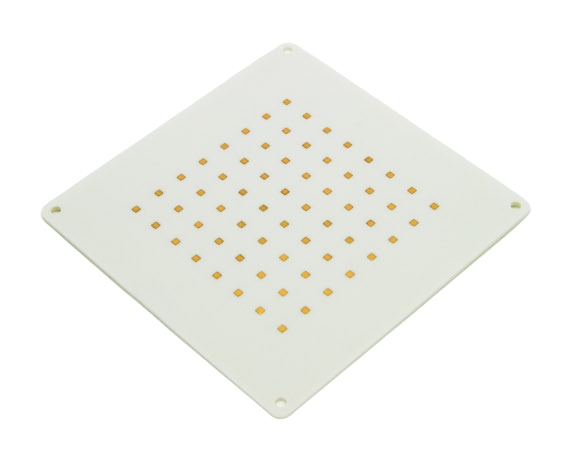
\includegraphics[width=\linewidth]{data/presentation/antenna-2.png}
  \end{minipage}
\end{figure}

\end{frame}


\begin{frame}
\frametitlecounted{Ներածություն}

Անտենաներում հայտնվող թերությունները բերում են անցանկալի խնդիրների, օրինակ՝
\begin{itemize}
    \item Ազդանշանների թուլացումներ կամ կորուստներ
    \item Ավելցուկային անցանկալի ինտերֆերենցիաներ
    \item Հաճախային շեղումներ
    \item Ազդանշանների աղավաղումներ
\end{itemize}
Ընդհանուր դեպքում՝ թերությունները ազդեցություն են թողնում անտենայից ճառագայթվող էլեկտրամագնիսական դաշտի վրա։

\end{frame}

\begin{frame}
\frametitlecounted{Ներածություն}

Էլեկտրամագնիսական դաշտը հետազոտելու միջոցներ՝

\begin{itemize}
    \item Սկանավորման տեխնիկա՝
        \begin{itemize}
            \item Սկանավորող ջերմային մանրադիտակ (Scanning thermal microscope (SThM))
            \item Մերձադաշտի սկանավորման օպտիկական մանրադիտակ (Near-field scanning optical microscope (NSOM))
        \end{itemize}
    \item Ջերմաառաձգական օպտիկական ինդիկատորով մանրադիտակ (ՋԱՕԻՄ)
\end{itemize}

\end{frame}

\resetCountingSlides{2}

\begin{frame}
\frametitlecounted{Առավելություններ և թերություններ}
    Սկանավորման տեխնիկայի առավելություններն են՝
    \begin{itemize}
        \item Մեծ տարածական լուծունակություն
    \end{itemize}
    Սկանավորման տեխնիկայի թերություններն են՝
    \begin{itemize}
        \item Պահանջում են թանկ և բարդ հասանելի նյութեր և սարքեր
        \item Չափումների խիստ պայմաններ
        \item Չափումների դանդաղ տևողություն
        \item SThM֊ը պահանջում է հպում չափվող նմուշի հետ
    \end{itemize}
\end{frame}

\begin{frame}
\frametitlecounted{Առավելություններ և թերություններ}
    ՋԱՕԻՄ֊ի առավելություններն են՝
    \begin{itemize}
        \item Մեծ տարածական լուծունակություն
        \item Մեծ ջերմային զգայունություն
        \item Պահանջվող սարքերը թանկ չեն և հեշտ հասանելի
        \item Աշխատում է առանց չափվող նմուշի հետ հպվելու
        \item Ալիքների չափման հաճախային տիրույթը ծածկում է ամբողջ էլեկտրամագնիսական սպեկտրը
    \end{itemize}
    ՋԱՕԻՄ֊ի թերություններն են՝
    \begin{itemize}
        \item Չափումների դանդաղ տևողություն
    \end{itemize}
\end{frame}


\resetCountingSlides{3}

\begin{frame}
\frametitlecounted{ՋԱՕԻՄ}
    ՋԱՕԻՄ֊ի սկզբունքային սխեման՝
    \begin{figure}
        \centering
        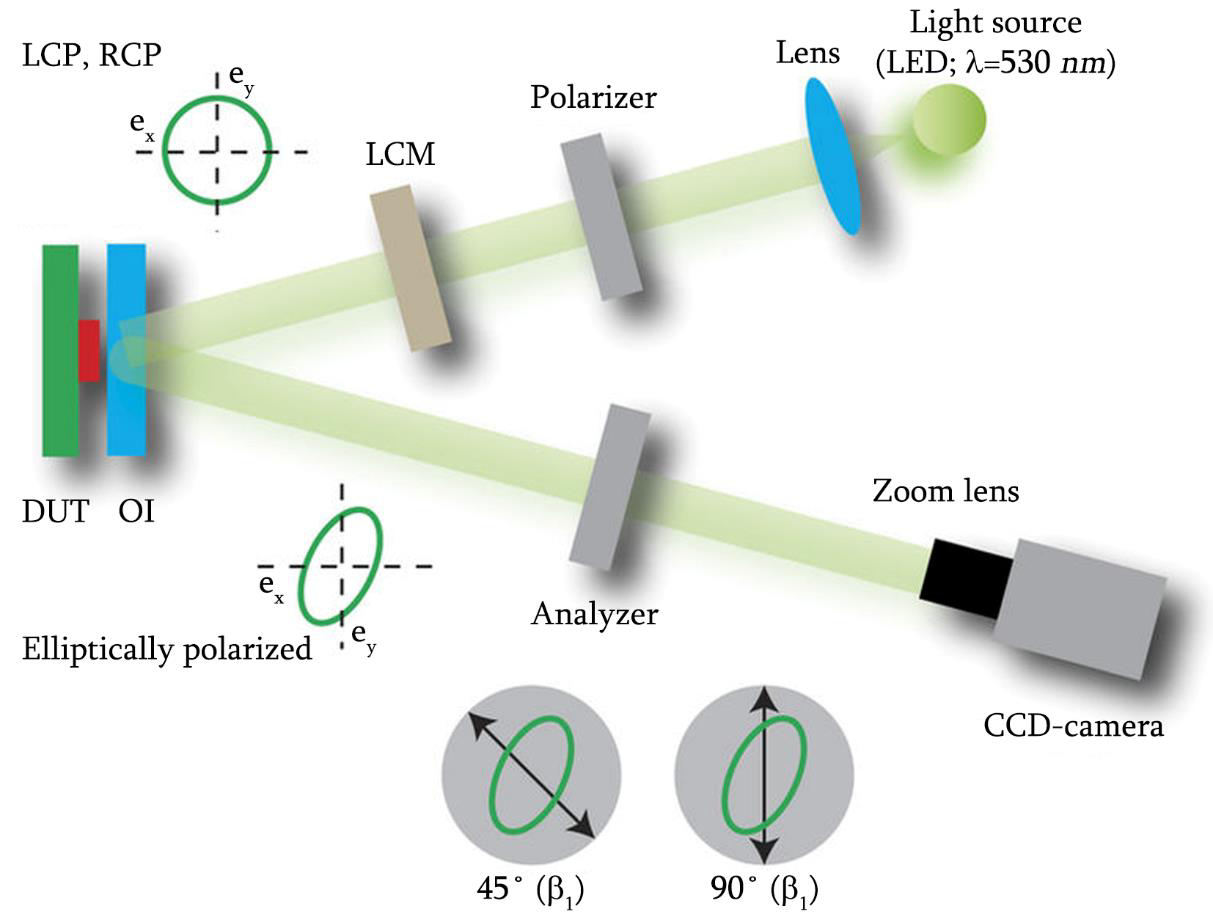
\includegraphics[width=0.9\textwidth]{data/TEOIM/0.jpg}
    \end{figure}
\end{frame}

\begin{frame}
\frametitlecounted{ՋԱՕԻՄ}
    Ֆոտոէլաստիկ երևույթը օպտիկական ինդիկատորում՝
    \begin{figure}
        \centering
        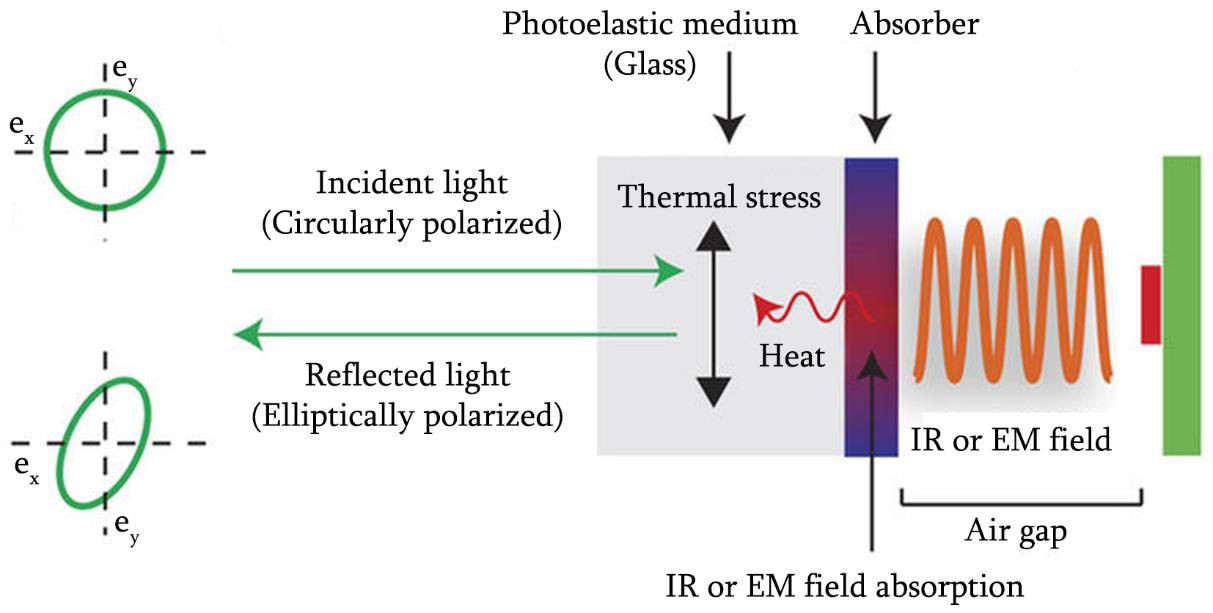
\includegraphics[width=\textwidth]{data/TEOIM/1.jpg}
    \end{figure}
\end{frame}

\begin{frame}
\frametitlecounted{ՋԱՕԻՄ}
    Կապը $q$ ջերմային բաշխվածության և $\beta_1$, $\beta_2$ գծային երկբեկման միջև՝
    \begin{flalign*}
    q &= \frac {\lambda}{2\pi dS} \frac{1 - \nu}{\alpha Ek}
    \left( 2 \frac{\partial^2 \beta_2}{\partial x \partial y} +  \frac{\partial^2 \beta_1}{\partial x^2} - \frac{\partial^2\beta_1}{\partial y^2} \right)
    \end{flalign*}
    {\fontsize{10}{10} \selectfont
        որտեղ՝ \\
        $S$֊ը լարման օպտիկական հաստատունն է, \\
        $\lambda$֊ն ընկնող լույսի ալիքի երկարությունն է, \\
        $d$֊ն ինդիկատորի հաստությունն է, \\
        $\alpha$֊ն ջերմային ընդարձակման գործակիցն է, \\
        $\nu$֊ն Պուասոնի գործակիցն է, \\
        $E$֊ն Յունգի մոդուլն է, \\
        $k$֊ն ինդիկատորի էֆեկտիվ ջերմահաղորդականությունն է։
    }
    
\end{frame}


\resetCountingSlides{6}

\begin{frame}
\frametitlecounted{Ալիքատարային անտենայի հետազոտումը}

{\fontsize{9}{9} \selectfont
    ՋԱՕԻՄ֊ի միջոցով հետազոտվել է ալիքատարային անտենայի էլեկտրամագնիսական ճառագայթումը։ Օգտագործվել է Pasternak արտադրության PE9804 WR-90 մոդելի ալիքատարը։
}
\begin{figure}
    \centering
    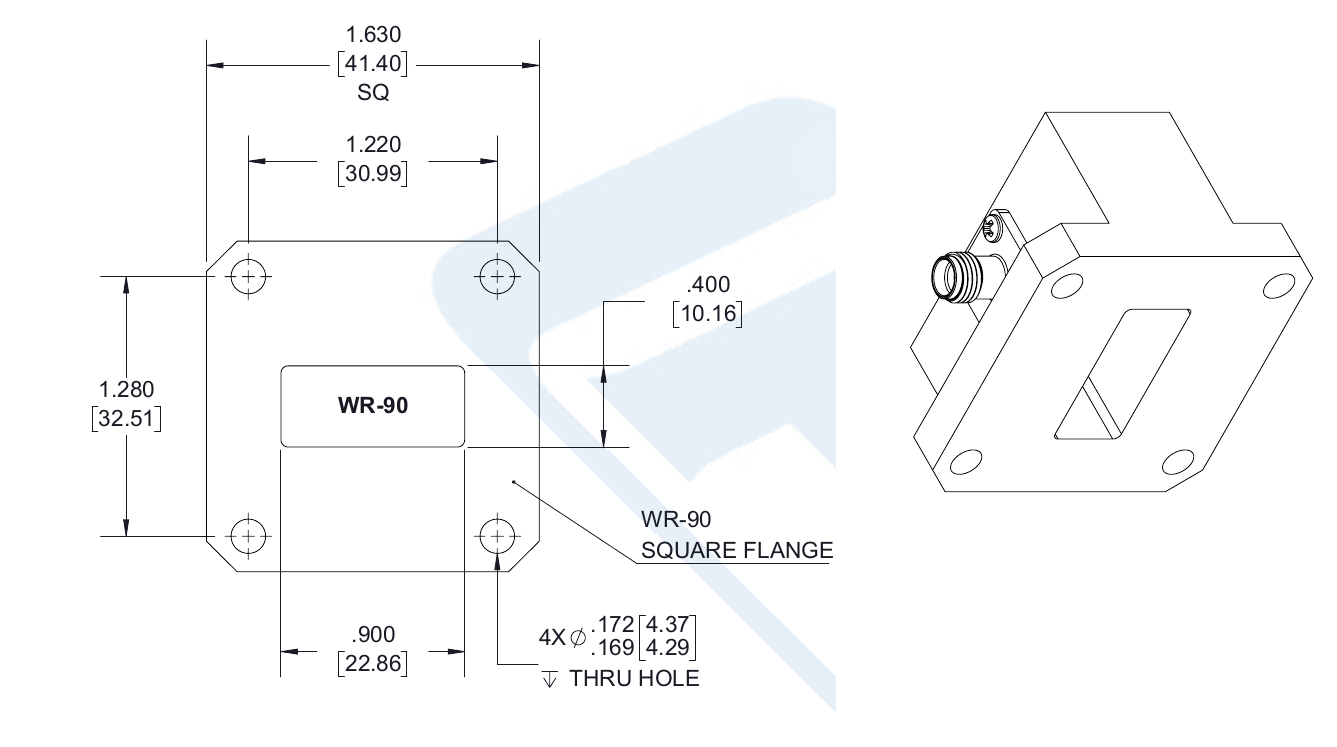
\includegraphics[width=0.9\textwidth]{data/presentation/waveguide-scheme.png}
\end{figure}

\end{frame}


\begin{frame}
\frametitlecounted{Ալիքատարային անտենայի հետազոտումը}

\begin{figure}[ht]
    \centering
    \begin{minipage}[c]{0.05\linewidth}
        \rotatebox{90}{0 dBm, 6-14 ԳՀց, մագնիսական դաշտ}
    \end{minipage}
    \hfill
    \begin{minipage}[c]{0.93\linewidth}
    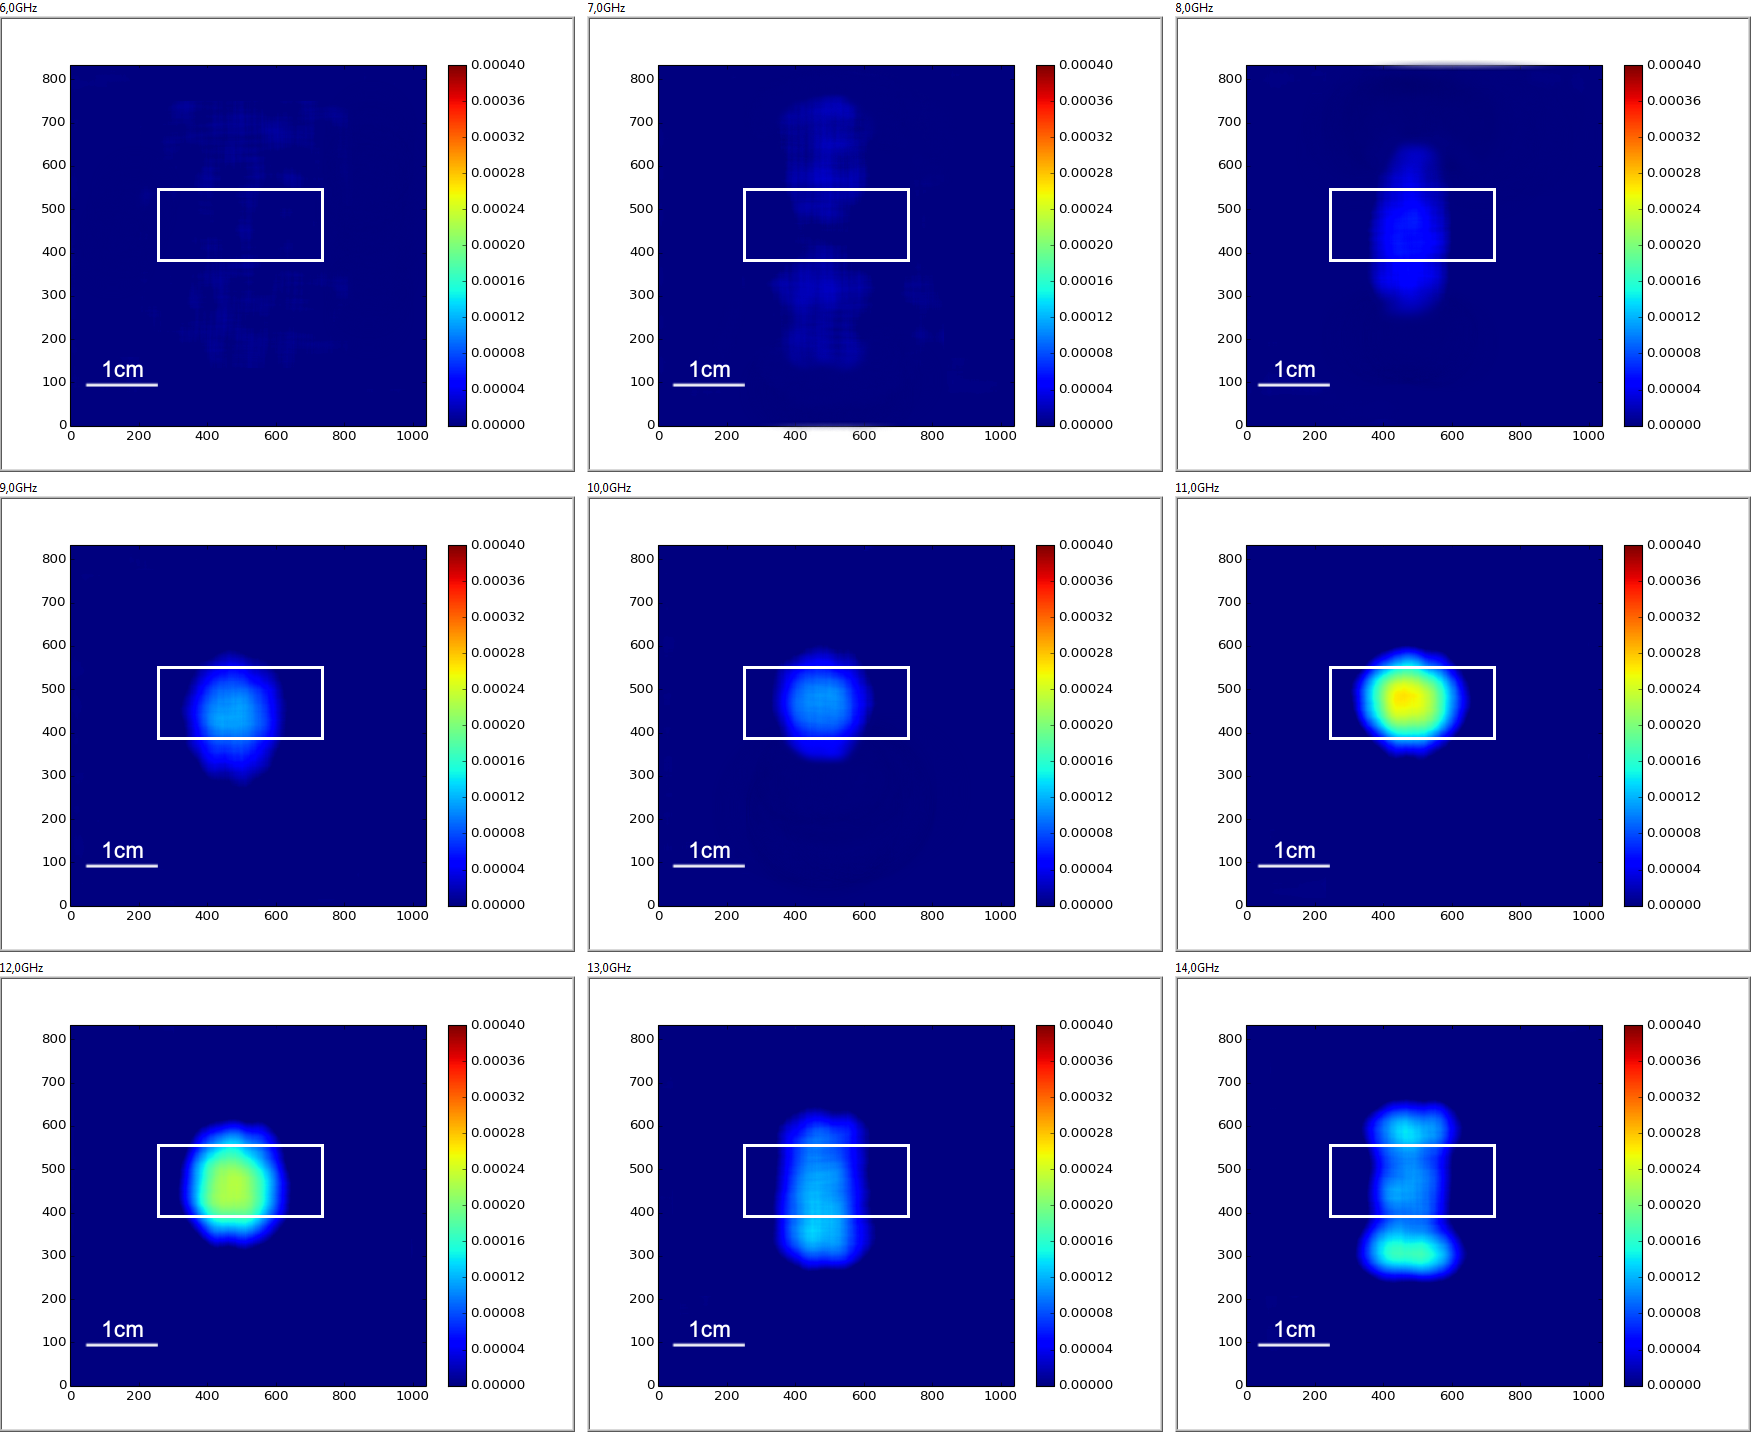
\includegraphics[width=\linewidth]{data/experiment-results/free field of antenna, 6-14ghz, 0dbm generator output, distance 5mm.png}
    \end{minipage}
\end{figure}

\end{frame}


\begin{frame}
\frametitlecounted{Ալիքատարային անտենայի հետազոտումը}

\begin{figure}[ht]
    \centering
    \begin{minipage}[c]{0.05\linewidth}
        \rotatebox{90}{3 dBm, 6-14 ԳՀց, մագնիսական դաշտ}
    \end{minipage}
    \hfill
    \begin{minipage}[c]{0.93\linewidth}
    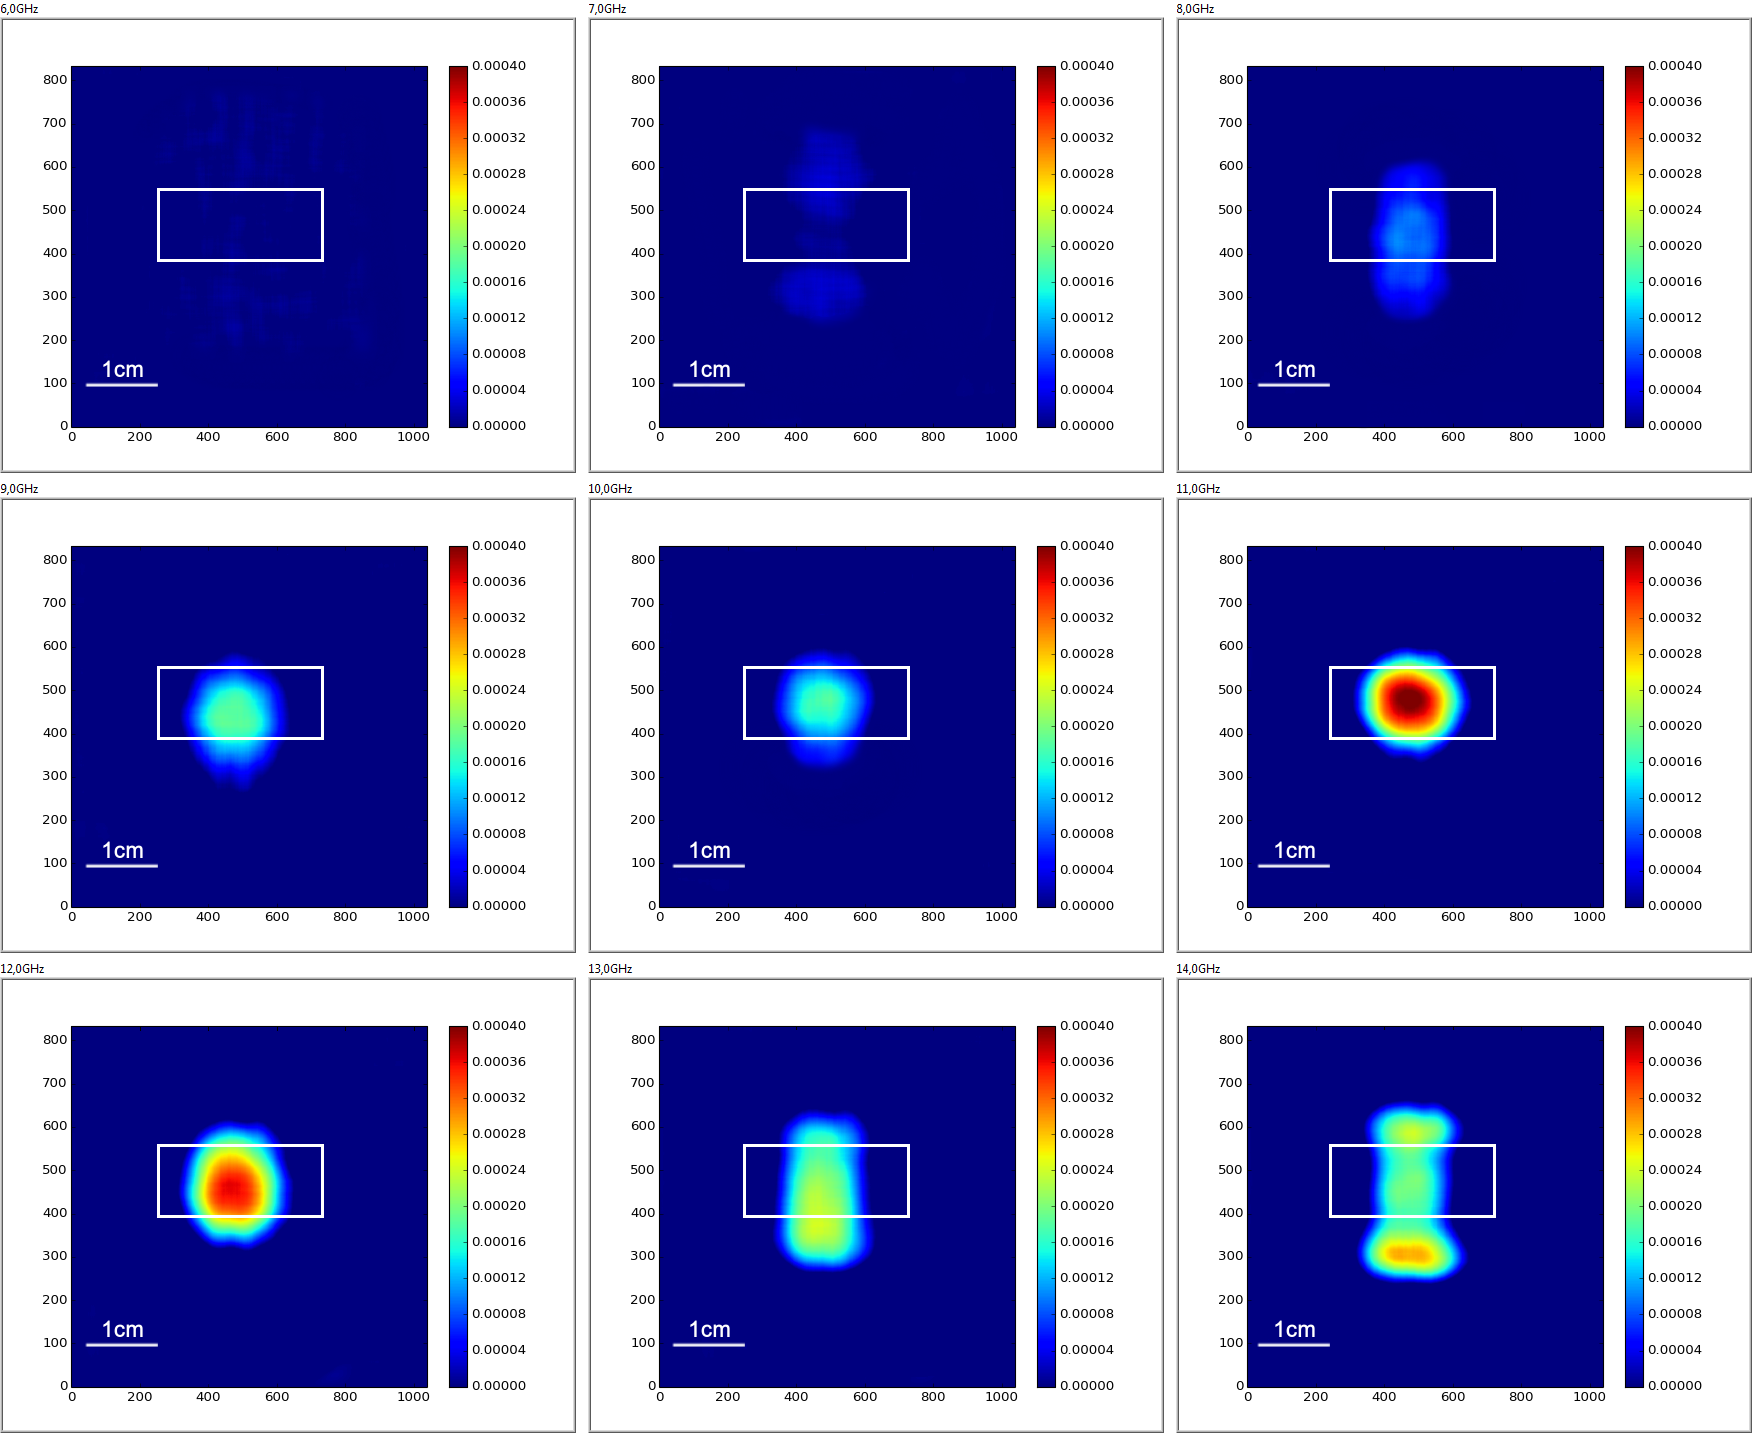
\includegraphics[width=\linewidth]{data/experiment-results/free field of antenna, 6-14ghz, 3dbm generator output, distance 5mm.png}
    \end{minipage}
\end{figure}

\end{frame}


\begin{frame}
\frametitlecounted{Ալիքատարային անտենայի հետազոտումը}

\begin{figure}[ht]
    \centering
    \begin{minipage}[c]{0.05\linewidth}
        \rotatebox{90}{6 dBm, 6-14 ԳՀց, մագնիսական դաշտ}
    \end{minipage}
    \hfill
    \begin{minipage}[c]{0.93\linewidth}
    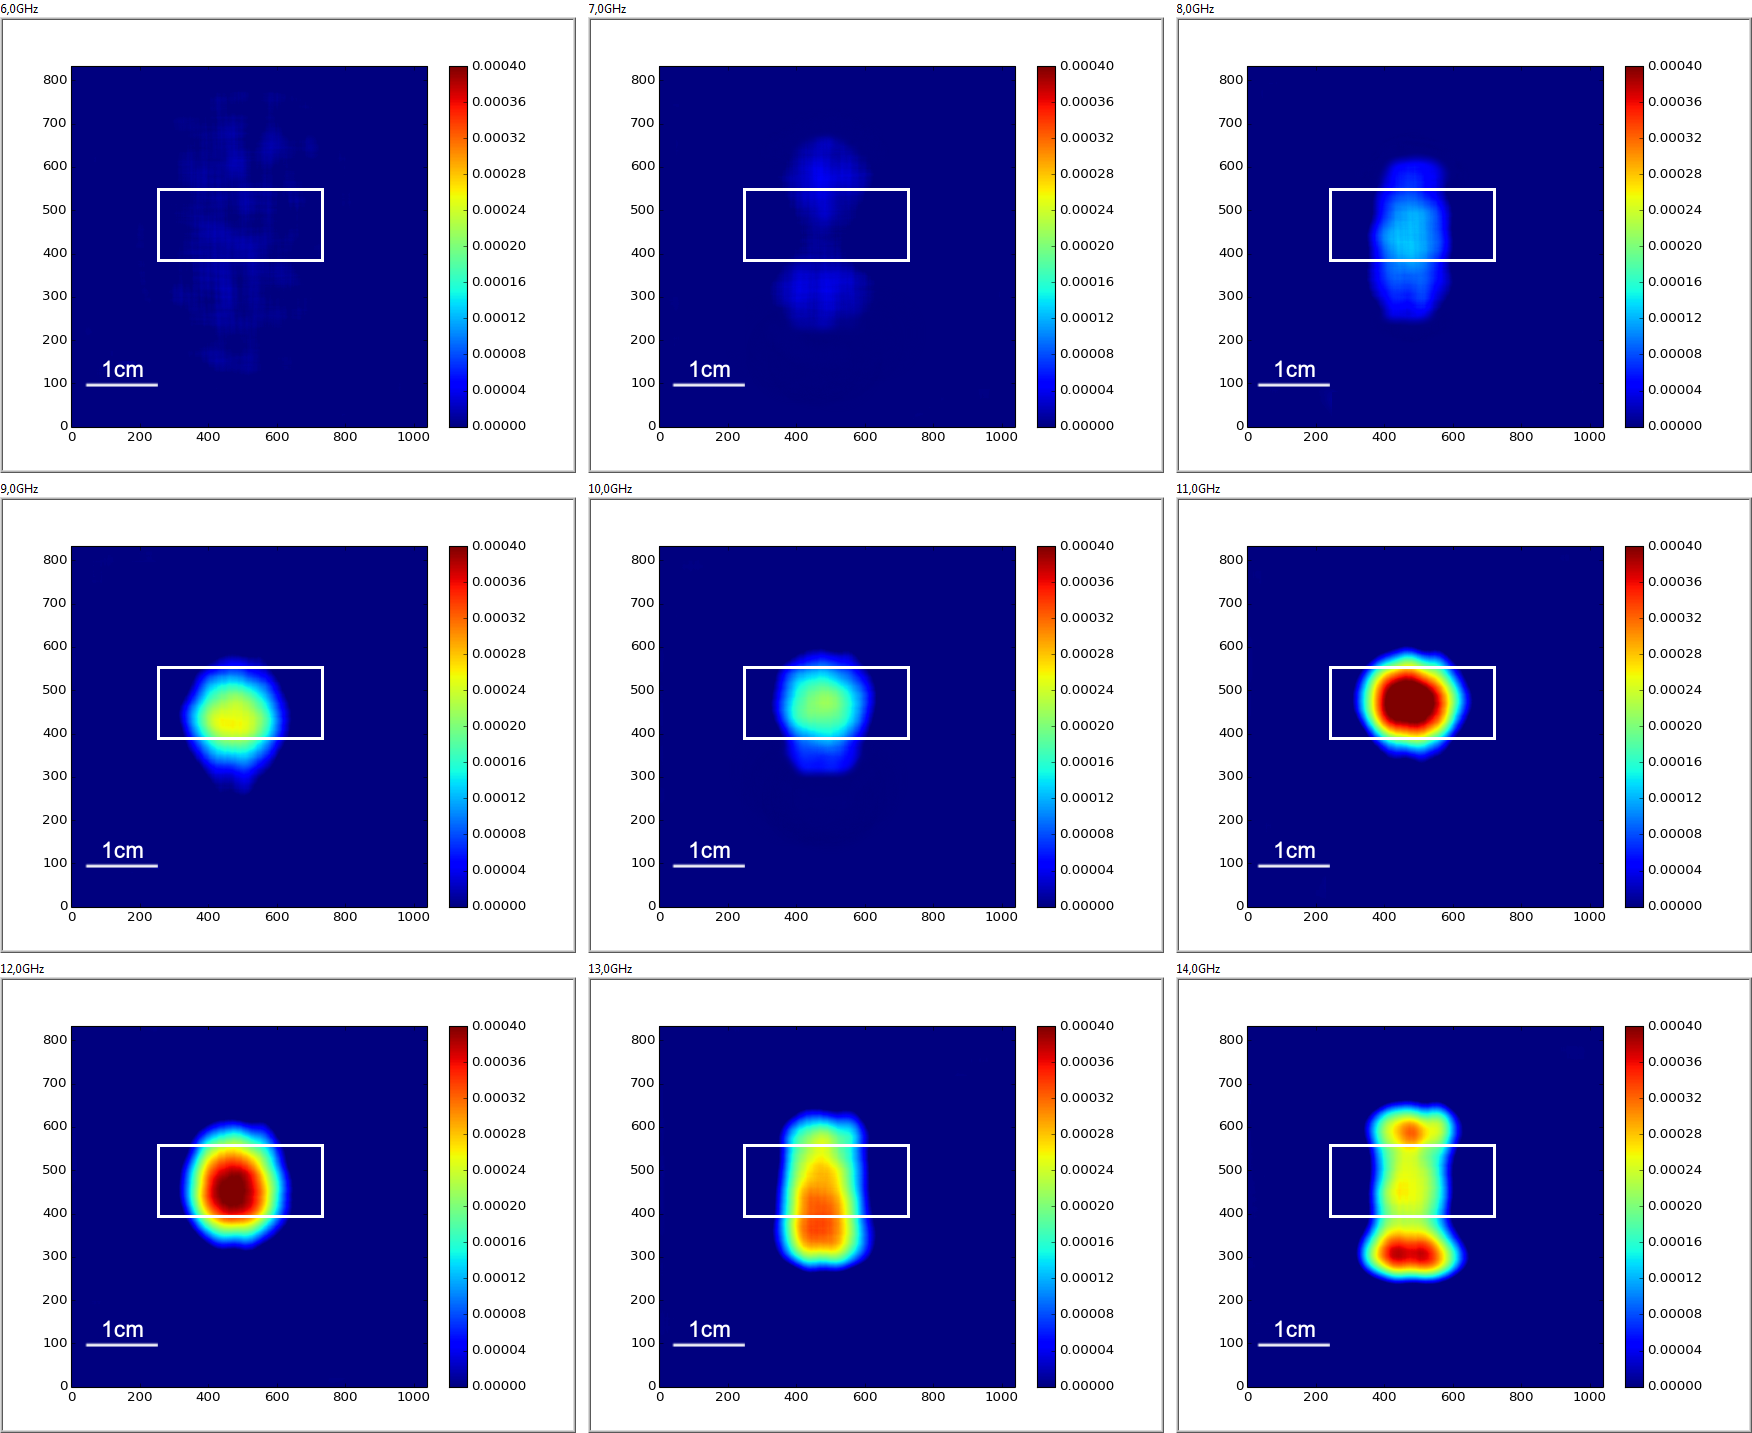
\includegraphics[width=\linewidth]{data/experiment-results/free field of antenna, 6-14ghz, 6dbm generator output, distance 5mm.png}
    \end{minipage}
\end{figure}

\end{frame}


\begin{frame}
\frametitlecounted{Ալիքատարային անտենայի հետազոտումը}

{\fontsize{10}{10} \selectfont Միջինացված ինտենսիվության կախումը հաճախությունից՝ յուրաքանչյուր մուտքային հզորության դեպքում։}

\begin{figure}[ht]
    \centering
    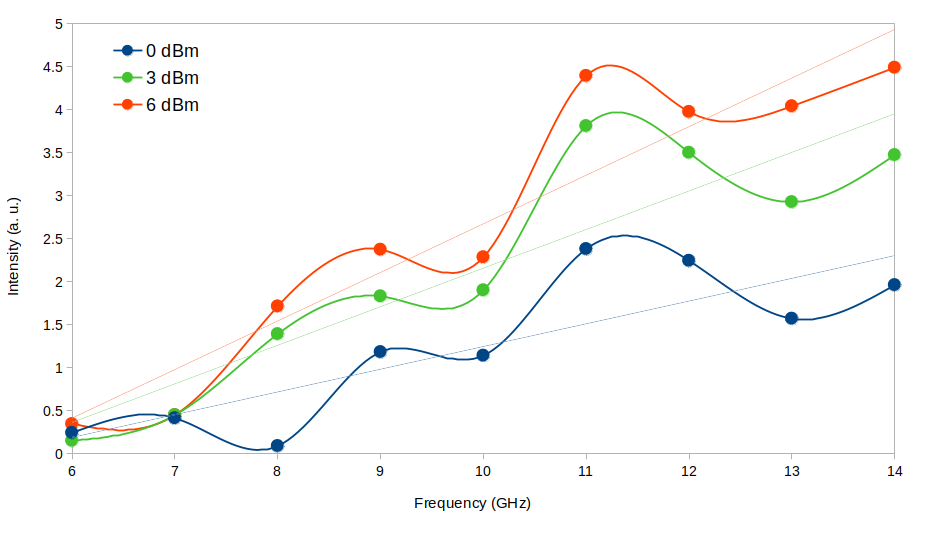
\includegraphics[width=\linewidth]{data/experiment-results/free_field_of_antenna_6-14GHz_0-6dBm_generator_output_distance_5mm.png}
\end{figure}

\end{frame}


\begin{frame}
\frametitlecounted{Ալիքատարային անտենայի հետազոտումը}

{\fontsize{10}{10} \selectfont Միջինացված ինտենսիվության կախումը մուտքային հզորությունից՝ 8, 11 և 12 ԳՀց հաճախությունների դեպքում։}

\begin{figure}[ht]
    \centering
    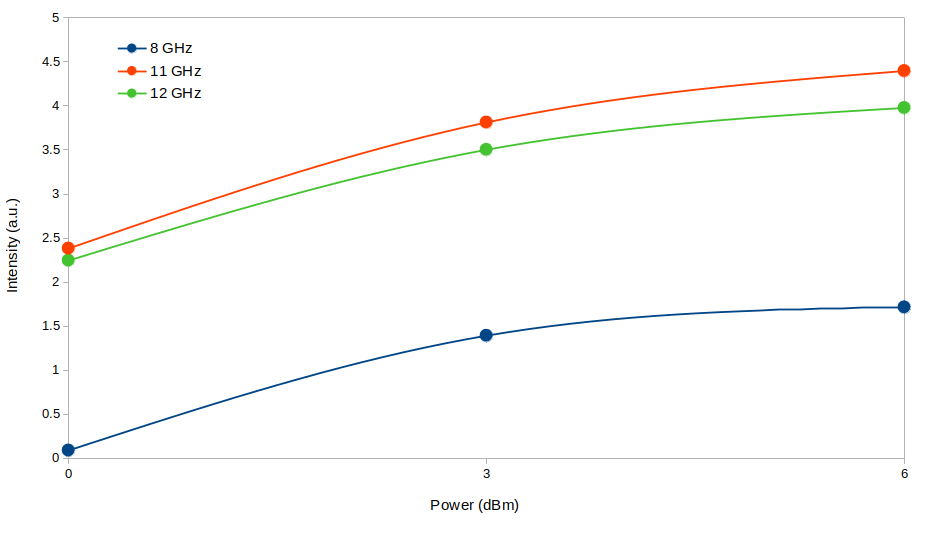
\includegraphics[width=\linewidth]{data/experiment-results/free_field_of_antenna_0-6dBm_8-11-12GHz_generator_output_distance_5mm.png}
\end{figure}

\end{frame}


\resetCountingSlides{1}

\begin{frame}
\frametitlecounted{Եզրակացություն}
    \begin{itemize}
        \item Հզորության մեծացմանը զուգընթաց դաշտի ինտենսիվությունն աճել է, բայց դաշտի բաշխվածության տեսքը չի փոխվել
        \item Հաճախության աճմանը զուգընթաց փոխվել է ինչպես դաշտի ինտենսիվությունը, այնպես էլ բաշխվածության տեսքը
        \item Առավելագույն ինտենսիվությունը գրանցվել է ալիքի 11 ԳՀց հաճախության դեպքում
    \end{itemize}
\end{frame}


\resetCountingSlides{1}

\newcommand{\bibfontsize}{\fontsize{8}{8} \selectfont}
\let\oldbibitem\bibitem
\renewcommand{\bibitem}[1]{\bibfontsize \oldbibitem{#1}}

\begin{frame}
\frametitlecounted{Գրականություն}

\renewcommand{\section}[2]{}

\setbeamertemplate{bibliography item}[text]
\begin{thebibliography}{9}

\bibitem{yue2012nanoscalethermal}
{\bibfontsize Yue, Y. \& Wang, X. Nanoscale thermal probing. Nano Reviews. 3, 11586 (2012).
}
\bibitem{xie1990picosecond}
{\bibfontsize Xie, X., Simon, J. D. Picosecond circular dichroism spectroscopy: a Jones matrix analysis. J. Opt. Soc. Am. B 7, 1673 (1990).
}
\bibitem{arakelyan2016teoim}
{\bibfontsize H. Lee, S. Arakelyan, B. Friedman, K. Lee, Temperature and microwave near field imaging by thermo-elastic optical indicator microscopy, Sci. Rep. 6, 39696 (2016).
}
\bibitem{barron2011thermalstress}
{\bibfontsize Barron R. F., Barron B. R. Design for Thermal Stresses. Ch. 6 (Wiley, 2011).
}
\bibitem{chen2013itofabcrication}
{\bibfontsize Chen Z, Li W, Li R, Zhang Y, Xu G, Cheng H. Fabrication of highly transparent and conductive indium-tin oxide thin films with a high figure of merit via solution processing. Langmuir. 2013 Nov 12;29(45):13836-42. doi: 10.1021/la4033282. Epub 2013 Oct 28. PMID: 24117323.
}

\end{thebibliography}

\end{frame}

\begin{frame}
\Huge \centering Շնորհակալություն
\end{frame}

\end{document}
